% 中文 TikZ 重排：坐标及曲线提取自原 PDF，未重新模拟数据。
\begin{figure}[htbp]
\centering
\definecolor{chfourfig4c0}{rgb}{0.13669,0.12195,0.12529}
\definecolor{chfourfig4c1}{rgb}{0.90323,0.90668,0.91019}
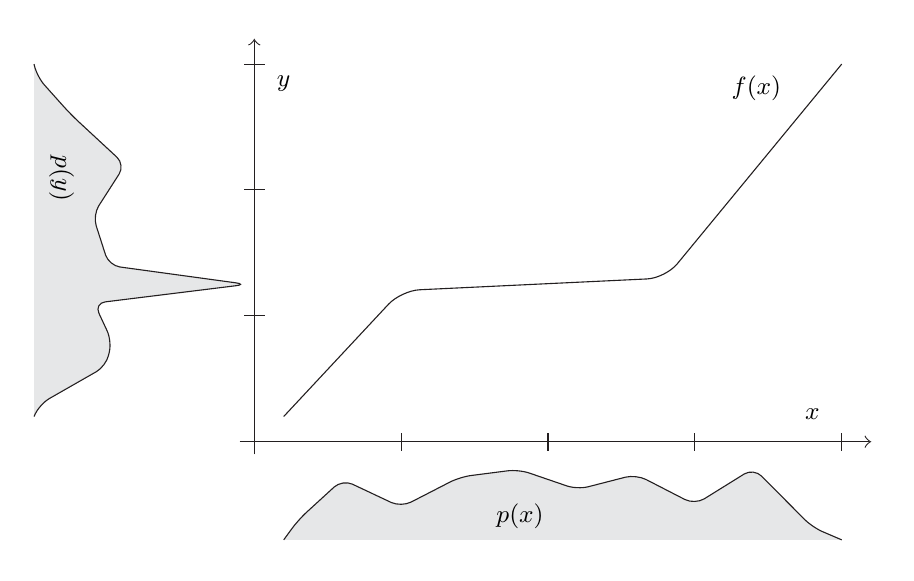
\begin{tikzpicture}[x=0.047cm,y=-0.047cm]
\useasboundingbox (0,0) rectangle (232,142);
\path[fill=none,draw=chfourfig4c0,line width=0.3985pt,draw opacity=1.0] (57.2782,111.8820) --(227.4671,111.8820);
\path[fill=none,draw=chfourfig4c0,line width=0.3188pt,draw opacity=1.0] (226.2716,110.2880) .. controls (226.3712,110.8857) and (227.4671,111.7824) ..(227.7660,111.8820) .. controls (227.4671,111.9816) and (226.3712,112.8783) ..(226.2716,113.4760);
\path[fill=none,draw=chfourfig4c0,line width=0.3985pt,draw opacity=1.0] (61.2470,115.2838) --(61.2470,3.4889);
\path[fill=none,draw=chfourfig4c0,line width=0.3188pt,draw opacity=1.0] (59.6530,4.6844) .. controls (60.2507,4.5848) and (61.1474,3.4889) ..(61.2470,3.1900) .. controls (61.3466,3.4889) and (62.2433,4.5848) ..(62.8410,4.6844);
\path[fill=none,draw=chfourfig4c0,line width=0.3985pt,draw opacity=1.0] (100.9324,114.2634) --(100.9324,109.5007);
\path[fill=none,draw=chfourfig4c0,line width=0.3985pt,draw opacity=1.0] (140.6177,114.2634) --(140.6177,109.5007);
\path[fill=none,draw=chfourfig4c0,line width=0.3985pt,draw opacity=1.0] (180.3031,114.2634) --(180.3031,109.5007);
\path[fill=none,draw=chfourfig4c0,line width=0.3985pt,draw opacity=1.0] (219.9884,114.2634) --(219.9884,109.5007);
\path[fill=none,draw=chfourfig4c0,line width=0.3985pt,draw opacity=1.0] (58.4688,77.8659) --(64.0253,77.8659);
\path[fill=none,draw=chfourfig4c0,line width=0.3985pt,draw opacity=1.0] (58.4688,43.8498) --(64.0253,43.8498);
\path[fill=none,draw=chfourfig4c0,line width=0.3985pt,draw opacity=1.0] (58.4688,9.8338) --(64.0253,9.8338);
\path[fill=none,draw=chfourfig4c0,line width=0.3985pt,draw opacity=1.0] (69.1839,105.0789) --(97.5277,74.7106) .. controls (99.4081,72.6960) and (103.1608,70.9568) ..(105.9098,70.8259) --(167.3887,67.8979) .. controls (170.1377,67.7671) and (173.7863,65.9365) ..(175.5382,63.8091) --(219.9884,9.8338);
\path[fill=chfourfig4c1,fill opacity=1.0,draw=chfourfig4c0,line width=0.3985pt,draw opacity=1.0] (69.1839,138.4145) --(71.3840,135.3973) .. controls (72.3608,134.0577) and (74.1424,132.0669) ..(75.3633,130.9507) --(82.8479,124.1080) .. controls (84.0687,122.9918) and (86.2695,122.6579) ..(87.7634,123.3622) --(98.2274,128.2952) .. controls (99.7213,128.9996) and (102.1244,128.9574) ..(103.5949,128.2011) --(114.1437,122.7758) .. controls (115.6142,122.0195) and (118.1348,121.2356) ..(119.7738,121.0249) --(129.7132,119.7471) .. controls (131.3522,119.5364) and (133.9477,119.8000) ..(135.5105,120.3358) --(145.7249,123.8380) .. controls (147.2878,124.3739) and (149.8528,124.4744) ..(151.4543,124.0626) --(161.5296,121.4716) .. controls (163.1310,121.0598) and (165.6212,121.3391) ..(167.0917,122.0954) --(177.6405,127.5206) .. controls (179.1110,128.2769) and (181.4403,128.1833) ..(182.8433,127.3114) --(193.6368,120.6042) .. controls (195.0397,119.7324) and (197.1213,119.9765) ..(198.2862,121.1496) --(209.9423,132.8887) .. controls (211.1072,134.0617) and (213.2852,135.5414) ..(214.8071,136.1937) --(219.9884,138.4145);
\path[fill=chfourfig4c1,fill opacity=1.0,draw=chfourfig4c0,line width=0.3985pt,draw opacity=1.0] (1.7190,105.0789) --(2.0393,104.3924) .. controls (2.7390,102.8928) and (4.4687,101.0128) ..(5.9028,100.1934) --(18.5684,92.9559) .. controls (20.0025,92.1364) and (21.4692,90.1681) ..(21.8445,88.5594) --(22.0728,87.5818) .. controls (22.4480,85.9731) and (22.1849,83.4534) ..(21.4852,81.9537) --(19.2572,77.1794) .. controls (18.5574,75.6798) and (19.3187,74.2999) ..(20.9577,74.0973) --(56.2951,69.7287) .. controls (57.9341,69.5261) and (57.9357,69.1804) ..(56.2988,68.9566) --(24.9222,64.6650) .. controls (23.2853,64.4412) and (21.5494,62.9852) ..(21.0450,61.4131) --(18.5061,53.4996) .. controls (18.0018,51.9274) and (18.3161,49.5259) ..(19.2082,48.1356) --(24.7084,39.5641) .. controls (25.6005,38.1738) and (25.3390,36.1341) ..(24.1241,35.0082) --(13.8399,25.4785) .. controls (12.6251,24.3526) and (10.7462,22.4404) ..(9.6432,21.2074) --(4.5100,15.4682) .. controls (3.4070,14.2351) and (2.2086,11.9315) ..(1.8332,10.3228) --(1.7190,9.8337);
\node[font=\small,inner sep=0pt,rotate=0] (ch04f4t0) at (69.1837,15.0379) {$y$};
\node[font=\small,inner sep=0pt,rotate=0] (ch04f4t1) at (212.0347,104.4399) {$x$};
\node[font=\small,inner sep=0pt,rotate=0] (ch04f4t2) at (196.9277,16.3515) {$f(x)$};
\node[font=\small,inner sep=0pt,rotate=0] (ch04f4t3) at (133.0587,132.0056) {$p(x)$};
\node[font=\small,inner sep=0pt,rotate=-90] (ch04f4t4) at (9.1484,40.8267) {$p(y)$};
\end{tikzpicture}
\caption{IGCI 思想的示意图：如果 $p_X$ 的选择独立于 $f$，那么，$p_Y$ 的峰往往出现在 $f$ 斜率较小、$f^{-1}$ 斜率较大的区域。因此，$p_Y$ 含有有关 $f^{-1}$ 的信息。IGCI 可以推广到 $f$ 不可微的情形［Janzing et al., 2015］。}
\label{fig:ch04-4}
\end{figure}
